%\documentclass[12pt]{article}
%\usepackage[a4paper, margin=1in]{geometry} 
%\usepackage{graphicx} 
%\usepackage{hyperref}
%\usepackage{float}
%\usepackage{multicol}
%\usepackage{multirow}
%\usepackage{amsmath}
%\usepackage[font=small, labelfont=bf]{caption}
%\usepackage[table,xcdraw]{xcolor}
%
%\begin{document}

%
% Evaluation of global alignment
%
\subsection{Evaluation of global alignment}
The underlying distribution of global alignment scores is unknown.

%
% Random generation of sequences
%
\subsubsection*{Random generation of sequences} 
One needs to consider using the appropriate length and compositions of amino acids or nucleotides needs when creating randomised sequences. \\

\noindent
\textbf{Example}

\noindent
Input sequences
\begin{verbatim}
    q: ACGT
    d: AGTACC  
\end{verbatim}

\noindent
Frequencies: {$f_{A}$ = 0.2, $f_{C}$ = 0.4, $f_{G}$ = 0.1, $f_{T}$ = 0.3} \\
Length: 6

\begin{verbatim}
    d1: CCAGTC
    d2: TCACCG
    d3: CTTGAA
    ...
\end{verbatim}

%
% Frequency distributions
%
\subsubsection*{Frequency distributions} 
\begin{itemize}
\item Universal (e.g. the whole protein database)
\item Global (e.g. protein super families)
\item Local (e.g. query and database sequences)
\end{itemize}

%
% Additional constrains
%
\subsubsection*{Additional constrains} 
Constrains on sequences generation are often considered. 
\begin{itemize}
\item Di-amino acid frequencies
\item Sub-region specific frequencies
\end{itemize}

%
% Non-parametric test and p-value
%
\subsubsection*{Non-parametric test and p-value} 
The simplest non-parametric test is calculating the rank of the score for the original alignment as the p-value. \\

$p=(b+1)/(n+1)$ \\

\noindent
where $b$ is the number of randomly generated scores above the score of the original alignment, and $n$ is the sample size. \\ 

\noindent
\textbf{N.B.} $n$ should be sufficiently large (e.g. $>$1000) to estimate an accurate p-value. \\

% NEWPAGE
\newpage

\noindent
\textbf{Example}

\begin{figure}[H]
  \centering
      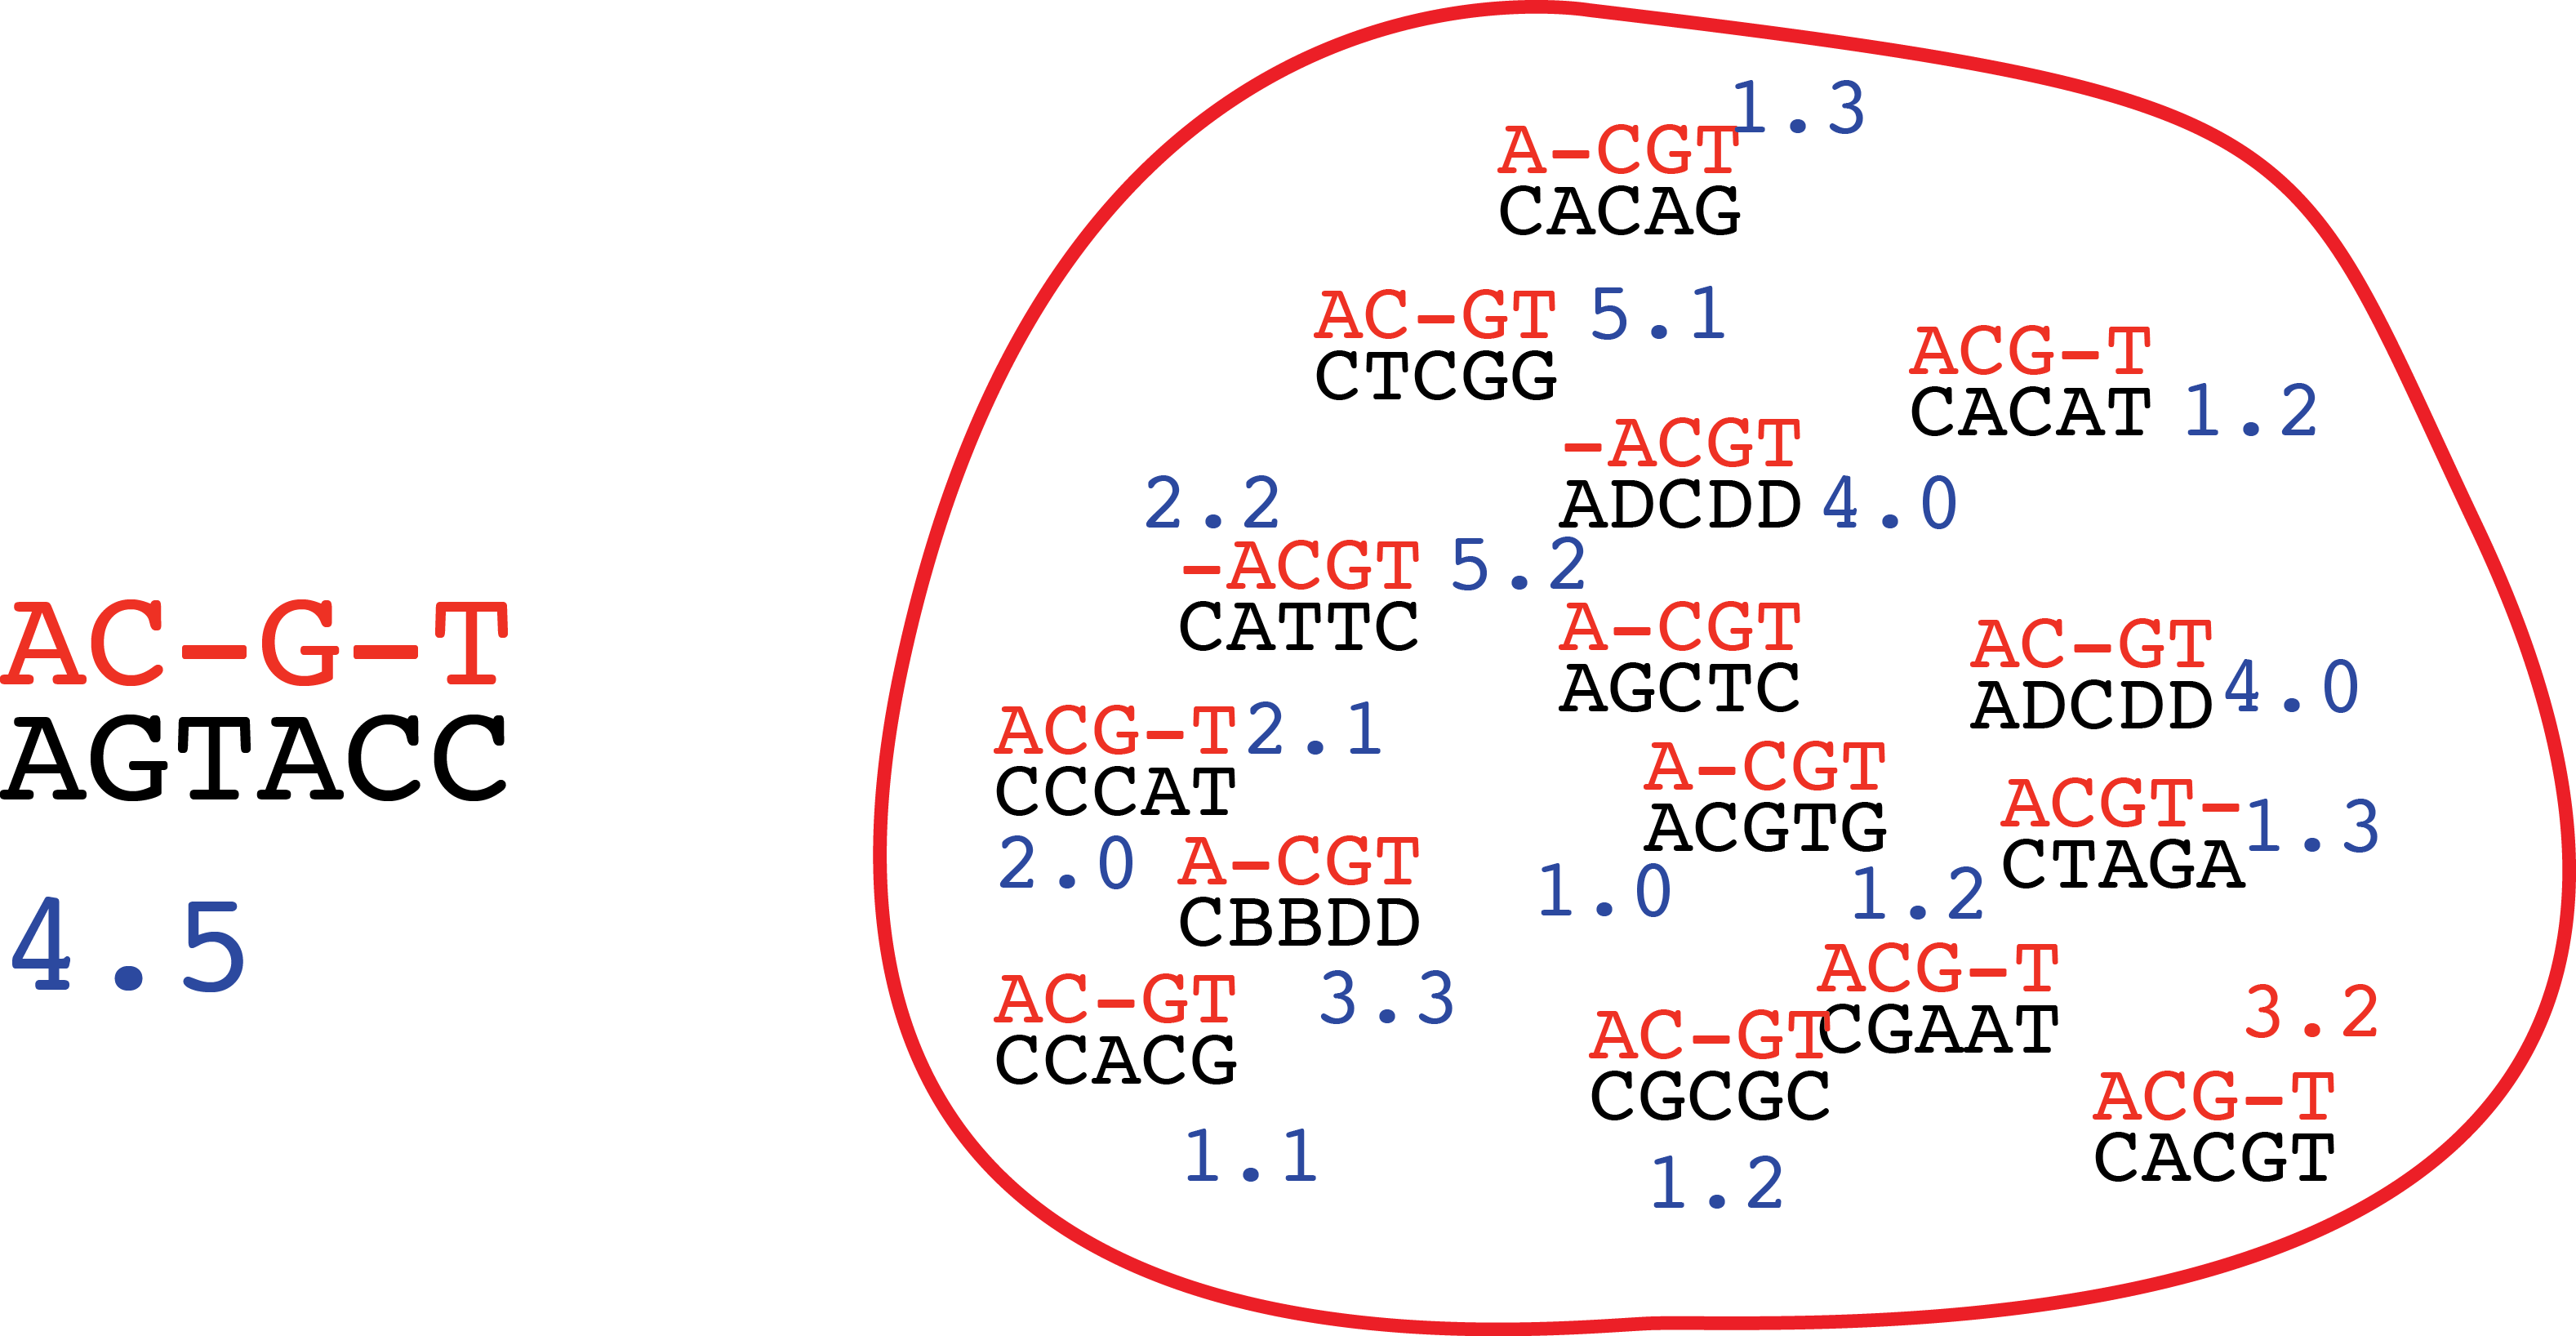
\includegraphics[width=0.5 \textwidth]{fig06/random_sequences.png}
  \caption{Randomly generated sequences and alignment scores}
\end{figure}

\begin{table}[H]
\centering
\tiny
\begin{tabular}{llllllllllllllllllll}
\hline
\multicolumn{1}{|l|}{1} & \multicolumn{1}{l|}{2}   & \multicolumn{1}{l|}{3}   & \multicolumn{1}{l|}{4}   & \multicolumn{1}{l|}{5}   & \multicolumn{1}{l|}{6}   & \multicolumn{1}{l|}{7}   & \multicolumn{1}{l|}{8}   & \multicolumn{1}{l|}{9}   & \multicolumn{1}{l|}{10}  & \multicolumn{1}{l|}{11}  & \multicolumn{1}{l|}{12} & \multicolumn{1}{l|}{13}  & \multicolumn{1}{l|}{14}  & \multicolumn{1}{l|}{15}  & \multicolumn{1}{l|}{16}  & \multicolumn{1}{l|}{17}  & \multicolumn{1}{l|}{18}  & \multicolumn{1}{l|}{19}  & \multicolumn{1}{l|}{20}  \\ \hline
\multicolumn{1}{|l|}{1} & \multicolumn{1}{l|}{1.1} & \multicolumn{1}{l|}{1.3} & \multicolumn{1}{l|}{1.4} & \multicolumn{1}{l|}{1.7} & \multicolumn{1}{l|}{2.1} & \multicolumn{1}{l|}{2.2} & \multicolumn{1}{l|}{2.2} & \multicolumn{1}{l|}{2.3} & \multicolumn{1}{l|}{2.5} & \multicolumn{1}{l|}{2.8} & \multicolumn{1}{l|}{3}  & \multicolumn{1}{l|}{3.2} & \multicolumn{1}{l|}{3.3} & \multicolumn{1}{l|}{3.4} & \multicolumn{1}{l|}{3.6} & \multicolumn{1}{l|}{4.2} & \multicolumn{1}{l|}{4.4} & \multicolumn{1}{l|}{4.7} & \multicolumn{1}{l|}{5.2} \\ \hline
                        &                          &                          &                          &                          &                          &                          &                          &                          &                          &                          &                         &                          &                          &                          &                          &                          & \multicolumn{2}{c}{\textbf{4.5}}                             &                         
\end{tabular}
\end{table}

p-value: $(2 + 1) / (20 + 1) = 0.1429$

\begin{itemize}
\item Significance level $\alpha = 0.2$:  reject the null hypothesis
\item Significance level $\alpha = 0.05$: the null hypothesis is not rejected
\end{itemize}

%
% Exercise \thesection.1
%
\subsubsection*{Exercise \thesection.1}

\begin{enumerate}
\item Calculate the frequencies of nucleotides from the four sequences below.

\begin{verbatim}
    d1: CCAGC
    d2: TCACG
    d3: CTTAA
    d4: AACAA
\end{verbatim}

Frequencies: \{$f_{A} = \quad$, $f_{C} = \quad$, $f_{G} =  \quad$, $f_{T} =  \quad$ \}

\item Calculate the p-value of the alignment below. 

\begin{verbatim}
    q: AACG
    d: A-CG
    Score: 40
\end{verbatim}

\noindent
Assume that the scores are pre-calculated for the alignments of the query sequence and nine randomly generated sequences as follows. Use them for the p-value calculation.

\begin{table}[H]
\centering
\small
\begin{tabular}{|l|l|l|l|l|l|l|l|l|l|}
\hline
\textbf{No.}   & 1 & 2  & 3  & 4  & 5  & 6  & 7  & 8  & 9  \\ \hline
\textbf{Score} & 4 & 14 & 33 & 45 & 74 & 76 & 82 & 83 & 94 \\ \hline
\end{tabular}
\end{table}


\end{enumerate}

%
% Using the normal distribution
%
\subsubsection*{Using the normal distribution}
The underlying distribution of global alignment scores is unknown, but the z-score is sometimes calculated. \\

\noindent
The z-score is: \\

$z = \dfrac{x-\mu}{\sigma}$ \\

\noindent
where: \\

$\mu$ is the mean of the population. \\

$\sigma$ is the standard deviation of the population.

%
% Mean and variacne
%
\subsubsection*{Mean and variance}
The sample mean ($\bar{x}$) and the sample variance ($s^2$) are calculated as follows. \\

$\bar{x} =\dfrac{1}{n} \sum_{i=1}^{n}x_{i}$ \\ \\

$s = \sqrt{\dfrac{\sum_{i=1}^{n}(x_{i}-\bar{x})^2}{n-1}}$

%
% Example of z-score
%
\subsubsection*{Example of z-score}

\begin{itemize}
\item $\bar{x}$: 2.78	
\item $s$: 1.4964
\end{itemize}

$z = \dfrac{4.5-2.78}{1.4964} = 1.1494$ \\

The p-value is 0.125196.

\bigskip 

%\end{document}
